\section{Truy xuất lai theo đồ thị tri thức}\label{sec:retrieval-design}
Truy xuất trong dạy học phục vụ bốn việc: chọn nội dung giảng tiếp theo, tìm căn cứ cho gợi ý, trả lời câu hỏi do học sinh đặt ra và giải thích một khái niệm. Cả bốn chịu hai ràng buộc mà truy xuất tổng quát không có. Ràng buộc phạm vi cấm dùng đoạn của bài chưa học để phản hồi, nhằm tránh dạy trước. Ràng buộc nền tảng chuyển những câu hỏi không có đoạn nguồn phù hợp cho giáo viên thay vì tạo thông tin không căn cứ. Hình~\ref{fig:retrieval-flow} tóm tắt luồng truy xuất.

\begin{figure}[H]
\centering
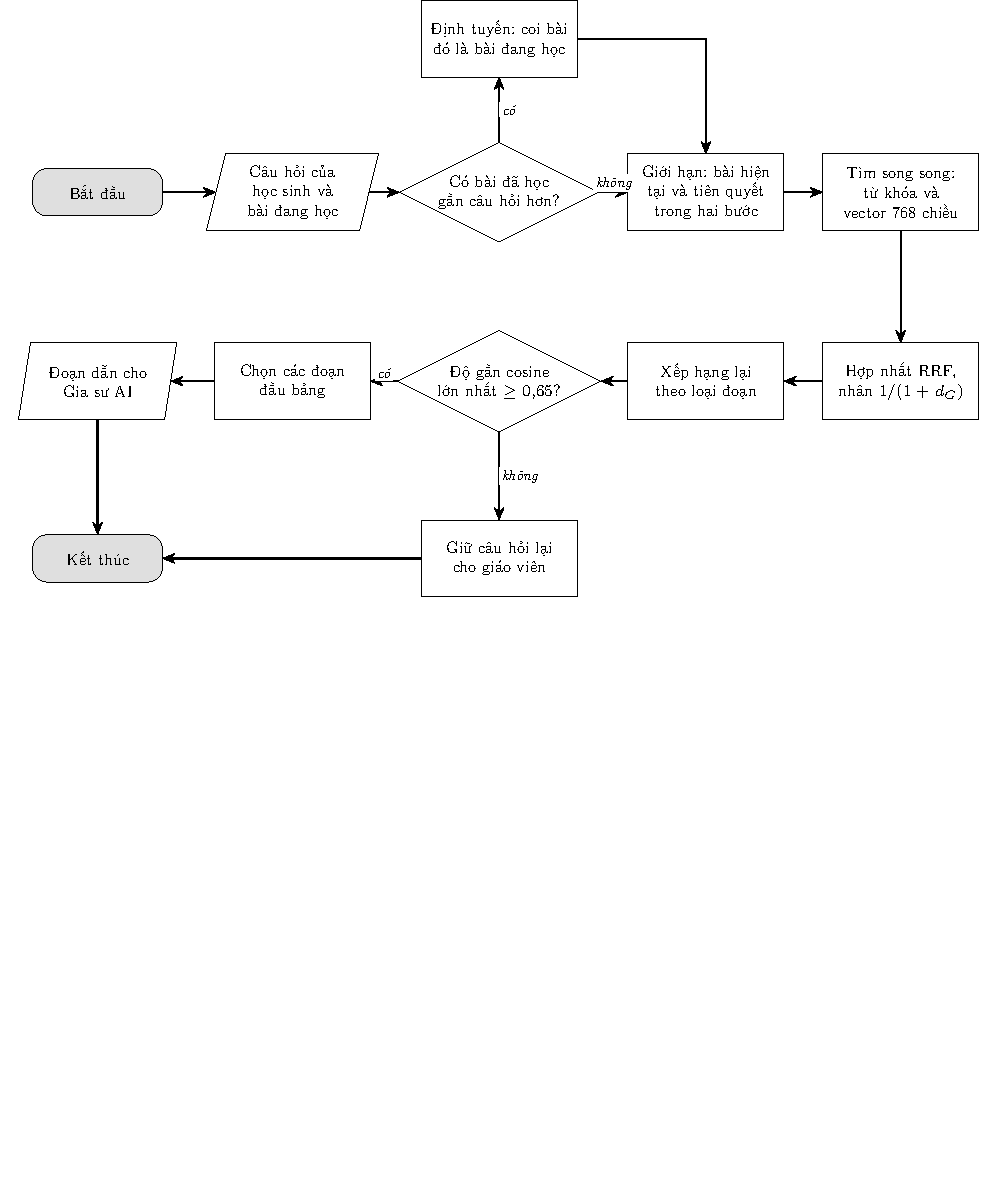
\includegraphics[width=\linewidth]{figures/pdf/fig-retrieval-flow.pdf}
\caption{Luồng truy xuất lai. Có hai cơ chế riêng của dạy học: định tuyến theo chủ đề (hình thoi đầu) và bước kiểm tra căn cứ (hình thoi sau, ngưỡng cosine $0{,}65$).}
\label{fig:retrieval-flow}
\end{figure}

\subsection{Phạm vi, từ khóa, ngữ nghĩa và hợp nhất}
Bước đầu giới hạn các đoạn được xét: phạm vi gồm bài học sinh đang học và các bài tiên quyết của nó cách không quá hai bước trên đồ thị, và một đoạn thuộc nhiều bài chỉ được xét khi mọi bài của nó nằm trong phạm vi. Bài sau bài đang học nằm ngoài phạm vi, nên câu trả lời không bao giờ dựa vào nội dung chưa dạy. Mỗi đoạn mang khoảng cách $d_G$ trên đồ thị từ bài đang học đến bài chứa nó.

Hai bộ xếp hạng chạy song song trong phạm vi. BM25 theo từ khóa chạy trên cả dạng có dấu và dạng bỏ dấu, dùng âm tiết và cặp âm tiết liền kề làm đơn vị vì tiếng Việt viết tách âm tiết và trẻ hay gõ không dấu. Bộ so khớp ngữ nghĩa dùng độ gần cosine giữa vector câu hỏi và vector $768$ chiều của đoạn do mô hình \texttt{gemini-embedding-001} tạo. Hai danh sách được hợp nhất bằng RRF (công thức~\eqref{eq:rrf}) rồi nhân với hệ số khoảng cách đồ thị:
\begin{equation}
\mathrm{fuse}(c)=\frac{1}{1+d_G(v,\nu(c))}\sum_{r\in\{\mathrm{BM25},\,\cos\}}\frac{1}{60+\mathrm{rank}_r(c)},
\label{eq:fuse}
\end{equation}
với $v$ là bài đang học và $\nu(c)$ là bài chứa đoạn $c$.

\subsection{Xếp hạng lại theo sư phạm}
Danh sách hợp nhất được xếp hạng lại: $\mathrm{score}(c)=\mathrm{fuse}(c)\,\kappa_m(\text{loại}_c)\,\gamma(c)$. Hệ số $\kappa_m\in[0{,}8;\,1{,}5]$ ưu tiên loại đoạn theo việc truy xuất đang phục vụ (khi giảng giải: lý thuyết $1{,}5$, ví dụ mẫu $1{,}1$, phương pháp $1{,}0$; khi gợi ý: phương pháp $1{,}4$, ví dụ mẫu $1{,}3$). Hệ số $\gamma$ theo ngữ cảnh bằng $1{,}5$ cho ghi chú lỗi sai vừa nhận diện, $1{,}6$ cho đoạn định nghĩa thuật ngữ được hỏi và $1$ trong các trường hợp còn lại; các đoạn đã dùng trong buổi bị hạ điểm để gia sư không lặp một cách giảng. Các hệ số này do người phát triển chọn thủ công theo nhu cầu của từng chế độ, không tinh chỉnh trên tập đánh giá và là diễn giải khai báo; mục~\ref{sec:eval-rag} đo độ nhạy của chúng và cho thấy việc đổi hệ số chưa làm đổi kết quả, nên các hệ số chưa được biện minh bằng dữ liệu. Cuối cùng hệ thống chọn các đoạn đứng đầu trong một ngân sách ký tự cố định, kèm vết các tín hiệu của từng đoạn để giáo viên xem được lý do một đoạn được chọn.

\subsection{Định tuyến theo chủ đề}
Phạm vi theo đồ thị có một hạn chế: học sinh thường hỏi lại khái niệm của bài trước khi đang học bài mới, và hệ số $1/(1+d_G)$ đẩy đoạn của bài hiện tại lên trước đoạn thật sự trả lời. Định tuyến theo chủ đề sửa điều này. Hệ thống so khớp câu hỏi với từng bài trong phạm vi bằng độ gần cosine lớn nhất; khi một bài trước gần câu hỏi hơn bài đang học quá một lề $\varepsilon=0{,}02$, các đoạn của bài đó được coi như có $d_G=0$. Định tuyến chỉ chọn bài tiên quyết đã học, nên không phá bất biến không dạy trước. Mục~\ref{sec:eval-rag} đo tác dụng của cơ chế này: bỏ định tuyến là điều làm mức truy xuất giảm nhiều nhất.

\subsection{Kiểm tra căn cứ và tra cứu ngoài kho}
Trước khi trả lời bằng nội dung của chương, hệ thống kiểm câu hỏi có căn cứ trong kho hay không. Câu được coi là có căn cứ khi độ gần cosine lớn nhất giữa câu hỏi và các đoạn chọn được đạt ngưỡng $0{,}65$, một diễn giải khai báo của đồ án. Câu nêu thuật ngữ Toán lớp 5 mà kho không dùng, như ``hình tròn'' hay ``thể tích'', bị coi là ngoài chương dù cosine vượt ngưỡng. Câu không có căn cứ được giữ lại cho giáo viên và gia sư kéo học sinh về câu đang làm.

Khi kho không có đoạn trả lời mà câu hỏi vẫn thuộc khái niệm của bài hiện tại hay nền trực tiếp của nó, hệ thống có thể tra một ấn phẩm công khai đã xác minh của nhà xuất bản giáo dục. Việc tra cứu chỉ gửi ra ngoài tên khái niệm chuẩn, không gửi lời hay tên học sinh, và nội dung trả về chỉ là căn cứ chứ không tự được nạp vào kho. Mô hình còn được giảng bằng kiến thức Toán chuẩn trong chủ đề hiện tại khi đoạn truy xuất không đủ, nhưng đoạn của giáo viên vẫn được ưu tiên và lời giảng phải qua kiểm nguồn và kiểm Toán.
